\documentclass[11pt,a4paper]{article}

\usepackage[utf8]{inputenc}
\usepackage[T1]{fontenc}
\usepackage[italian]{babel}
\usepackage{amsmath, amssymb}
\usepackage{geometry}
\usepackage{booktabs}
\usepackage{array}
\usepackage{graphicx}
\usepackage{hyperref}
\usepackage{xcolor}
\usepackage{enumitem}
\usepackage{caption}

\geometry{margin=2.5cm}
\hypersetup{colorlinks=true, linkcolor=blue, urlcolor=blue}

\title{Da 191 a 25 covariate: un modello lineare parsimonioso e\\
  interpretabile per l'Italian Fragility Composite Index}
\author{Progetto di Statistica Applicata --- Report di estensione}
\date{}

\begin{document}
\maketitle

\begin{abstract}
\noindent
Questo report documenta un'iterazione del benchmark lineare per
l'IFC realizzata in risposta al feedback del docente. Il primo
benchmark, con 191 covariate selezionate da LASSO, raggiungeva un
R$^{2}$ out-of-sample di $0{,}825$, ma era troppo denso per essere
discusso in modo sostantivo. Abbiamo quindi derivato un modello
parsimonioso in tre passi espliciti: eliminazione iterativa della
multicollinearit\`a tramite Variance Inflation Factor, selezione
delle top-N covariate per effetto standardizzato, e un filtro di
significativit\`a che sostituisce qualsiasi coefficiente non
significativo con il candidato successivo del ranking. Su richiesta
esplicita del docente, l'estensione del comune (superficie totale)
\`e stata esclusa a monte, perch\'e \`e un descrittore statico e non
un driver di fragilit\`a una volta che tutto il resto del modello
\`e espresso in densit\`a pro-capite. Il modello finale ha 25
covariate, tutte significative a $p < 10^{-6}$, con VIF massimo di
$6{,}4$. Il suo R$^{2}$ out-of-sample \`e $0{,}784$: una perdita
controllata di $0{,}041$ rispetto al benchmark a 191 covariate.
L'estensione con linear mixed model con random intercept annidato
regione/provincia recupera quasi tutta la perdita, raggiungendo
R$^{2} = 0{,}818$, solo $0{,}007$ sotto il benchmark originale. Il
test di Moran sui residui rileva ancora una autocorrelazione
spaziale positiva significativa ($I = 0{,}234,\ p < 0{,}001$),
confermando che la struttura spaziale \`e intrinseca alla
fragilit\`a comunale italiana e non un artefatto del set di
covariate. Diagnostiche aggiuntive su calibrazione, incertezza
predittiva e normalit\`a dei residui completano la valutazione e
sono discusse in sezioni dedicate.
\end{abstract}

\section*{Perch\'e questa estensione era necessaria}

Dopo la presentazione del primo benchmark il docente ha sollevato
quattro punti:
\begin{itemize}[leftmargin=2em]
  \item \textbf{troppe covariate}: 191 \`e illeggibile in un poster o
    in una singola slide; il range gestibile per un pubblico \`e
    10--20;
  \item \textbf{multicollinearit\`a}: il primo report aveva solo una
    nota qualitativa su PM$_{10}$/PM$_{2{,}5}$; un'analisi VIF
    sistematica avrebbe detto quante delle 191 sono predittori
    realmente indipendenti;
  \item \textbf{ridge vs lasso}: un confronto Elastic Net su diversi
    parametri di mix avrebbe chiarito se la scelta del
    regolarizzatore guida il risultato;
  \item \textbf{superficie}: la variabile
    \texttt{Superficie\_totale\_Kmq} \`e una caratteristica statica
    del comune e non dovrebbe apparire in un modello di fragilit\`a
    dove ogni altro conteggio \`e gi\`a stato normalizzato a densit\`a
    pro-capite.
\end{itemize}
Questa estensione risponde a tutti e quattro. Il confronto
numerico con il run originale a 191 covariate \`e esplicito in
tutto il documento.

% ================================================================
\section{Specificazione dei modelli}
% ================================================================

Usiamo quattro varianti di modello annidate. Nell'intero documento
$i$ indica l'osservazione comune $\times$ anno e $j$ la covariata.
I predittori $X_{ji}$ sono standardizzati, quindi $\hat\beta_j$ \`e
la variazione attesa di IFC associata a un aumento di una
deviazione standard della covariata $j$.

\paragraph{Linear model parsimonioso (LM).}
Baseline con 25 covariate fisse:
\begin{equation}
  \mathrm{IFC}_i \;=\; \beta_0 + \sum_{j=1}^{25} \beta_j X_{ji}
                       + \varepsilon_i,
  \qquad \varepsilon_i \sim \mathcal{N}(0,\sigma^2).
  \label{eq:lm}
\end{equation}

\paragraph{Random intercept di regione ($M_{\mathrm{geo}}$).}
Aggiunge un livello base per regione:
\begin{equation}
  \mathrm{IFC}_i \;=\; \beta_0 + \sum_{j=1}^{25} \beta_j X_{ji}
                       + u_{r(i)} + \varepsilon_i,
  \qquad u_r \sim \mathcal{N}(0,\sigma_R^2),
  \label{eq:geo}
\end{equation}
dove $r(i) \in \{1,\dots,20\}$ \`e la regione del comune $i$.
Il termine $u_{r(i)}$ \`e la fragilit\`a residua media della regione
$r$ che i fixed effects non riescono a spiegare.

\paragraph{Random intercept regione/provincia annidato ($M_{\mathrm{geo,nested}}$).}
Aggiunge un secondo livello a livello provinciale:
\begin{equation}
  \mathrm{IFC}_i \;=\; \beta_0 + \sum_{j=1}^{25} \beta_j X_{ji}
                       + u_{r(i)} + v_{p(i)\mid r(i)} + \varepsilon_i,
  \qquad v_{p\mid r} \sim \mathcal{N}(0,\sigma_P^2),
  \label{eq:geo_nested}
\end{equation}
con $p(i)$ una delle $107$ province. Ogni provincia ha la propria
fragilit\`a residua sopra quella regionale.

\paragraph{Random intercept di macroclasse GRINS ($M_{\mathrm{tax}}$).}
Sostituisce la gerarchia geografica con la tassonomia GRINS:
\begin{equation}
  \mathrm{IFC}_i \;=\; \beta_0 + \sum_{j=1}^{25} \beta_j X_{ji}
                       + t_{m(i)} + \varepsilon_i,
  \qquad t_m \sim \mathcal{N}(0,\sigma_T^2),
  \label{eq:tax}
\end{equation}
dove $m(i) \in \{\text{Italia interna},\text{Italia di mezzo},
\text{Italia metropolitana}\}$ \`e la macroclasse GRINS.

\paragraph{Regione $+$ macroclasse incrociati ($M_{\mathrm{geo+tax}}$).}
Combina regione e macroclasse come due random intercepts incrociati.
Verifica se la tassonomia aggiunge qualcosa oltre alla geografia
quando entrambe sono nel modello:
\begin{equation}
  \mathrm{IFC}_i \;=\; \beta_0 + \sum_{j=1}^{25} \beta_j X_{ji}
                       + u_{r(i)} + t_{m(i)} + \varepsilon_i.
  \label{eq:geo_plus_tax}
\end{equation}

% ================================================================
\section{Metodo}
% ================================================================

\subsection{Pruning via Variance Inflation Factor}

Per un modello lineare con $p$ predittori,
\begin{equation}
  \mathrm{VIF}_j \;=\; \frac{1}{1 - R^{2}_{j}},
  \quad
  R^{2}_{j} = R^{2}\!\left(X_j \sim X_{-j}\right),
\end{equation}
\`e la quota di varianza di $X_j$ gi\`a spiegata dagli altri
predittori. $\mathrm{VIF}=1$ corrisponde a indipendenza perfetta;
$\mathrm{VIF}>10$ \`e la soglia convenzionale di seria
collinearit\`a.

Partendo dalle 191 covariate selezionate da LASSO (esclusa a monte
la superficie), eliminiamo iterativamente la covariata con il VIF
massimo e rifittiamo. La procedura si ferma dopo \textbf{34}
iterazioni quando il VIF massimo scende sotto $10$. I peggiori
hanno VIF oltre cento (es.\ \texttt{mef\_tot\_classi\_amm},
$\mathrm{VIF}=159$). Il log completo \`e in
\verb|outputs/parsimonious_model/vif_drop_log.csv|.

\subsection{Ranking e selezione per effetto standardizzato}

Sulle 157 covariate VIF-pulite fittiamo un modello lineare con
predittori standardizzati e le ordiniamo per
$\lvert\hat\beta_j\rvert$. La standardizzazione rende i coefficienti
direttamente confrontabili tra variabili eterogenee. Le prime
$n=25$ formano il set candidato.

\subsection{Filtro di significativit\`a}

Quando rifittiamo le top-25 per $|\hat\beta|$, occasionalmente una
non risulta significativa: il suo $|\hat\beta|$ era guidato da una
residua collinearit\`a che la soglia VIF di 10 non aveva eliminato
del tutto. Lo script rimuove automaticamente i coefficienti con
$p > 0{,}05$ e li sostituisce con il candidato successivo del
ranking, poi rifitta e ripete finch\'e o tutte le 25 sono
significative o il pool di candidati \`e esaurito. Nel nostro run
\`e bastata una sostituzione.

\subsection{Estensione mixed-model e diagnostica spaziale}

Rifittiamo le quattro varianti mixed-model della Sezione~1 sul
nuovo set di 25 covariate, e ricalcoliamo il Moran's $I$ sui residui
di $M_{\mathrm{geo,nested}}$. I pesi spaziali sono il grafo
simmetrico ai 5 vicini pi\`u prossimi usato in precedenza.

\subsection{Cross-check Elastic Net}

Per rispondere alla domanda "LASSO con penalit\`a Ridge", Elastic
Net viene fittato sulle 157 covariate VIF-pulite per
$\alpha \in \{0{,}10\ 0{,}25\ 0{,}50\ 0{,}75\ 1{,}00\}$. $\alpha=1$
\`e LASSO puro; $\alpha=0$ sarebbe Ridge puro (senza selezione).

% ================================================================
\section{Risultati}
% ================================================================

\subsection{Parsimonia vs accuratezza}

La Figura~\ref{fig:tradeoff} mostra la curva di trade-off ottenuta
correndo cross-validation panel-aware su dimensioni del top-$n$ da 5
fino a tutti i 157 predittori VIF-puliti.

\begin{figure}[h!]
  \centering
  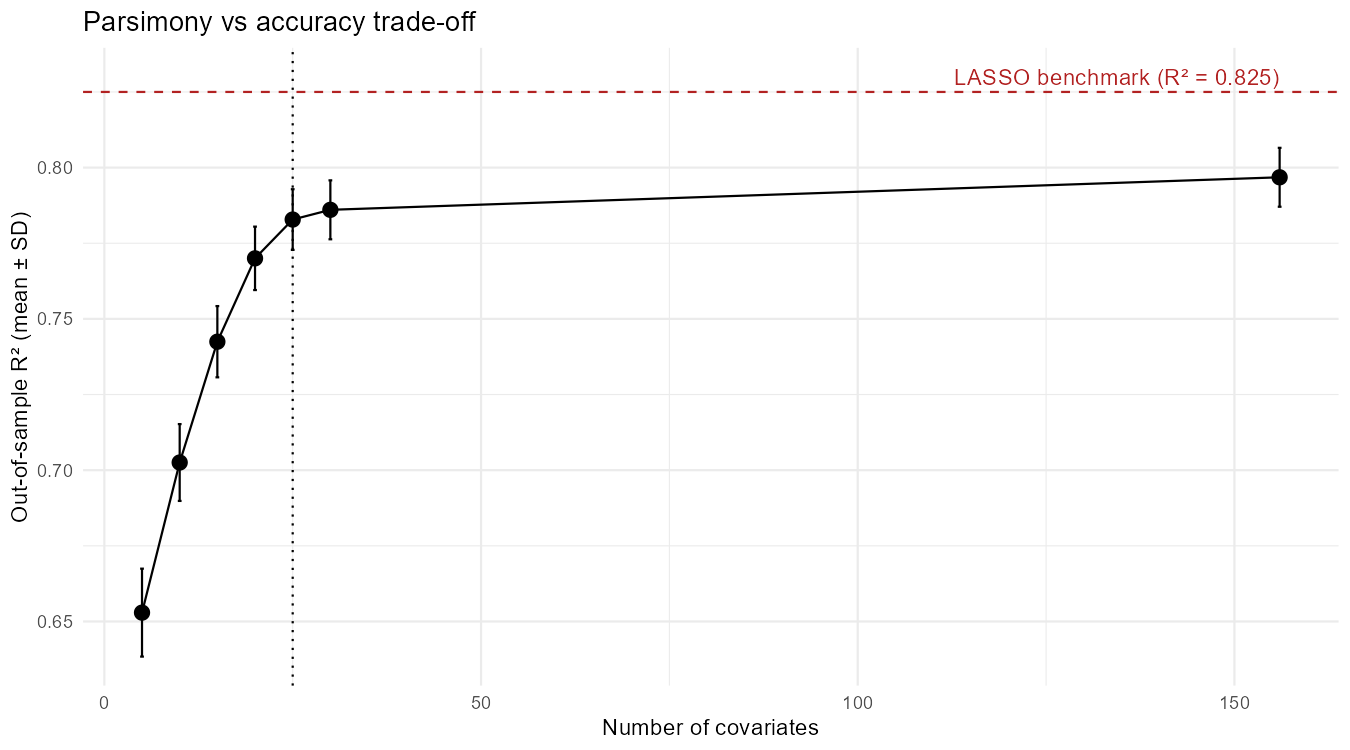
\includegraphics[width=0.80\textwidth]{figures/tradeoff_curve.png}
  \caption{R$^{2}$ out-of-sample in funzione del numero di covariate
    mantenute dal ranking VIF-pulito. Ogni punto \`e la media su 25
    fold di cross-validation panel-aware; le barre d'errore sono
    $\pm 1$ deviazione standard tra fold. La linea rossa
    tratteggiata segna l'R$^{2}$ del benchmark originale a 191
    covariate; la linea verticale punteggiata segna il nostro
    $n_{\text{final}}=25$. Il "gomito" della curva sta tra 20 e 25:
    spostarsi da 25 a 30 guadagna solo $+0{,}004$ di R$^{2}$, mentre
    spostarsi da 25 a 15 costa circa $0{,}03$.}
  \label{fig:tradeoff}
\end{figure}

\subsection{Il modello a 25 covariate e la sua lettura sostantiva}

Dopo il filtro di significativit\`a, tutti i 25 coefficienti sono
significativi a $p < 10^{-6}$ e il VIF massimo del modello finale
\`e $6{,}42$. La Tabella~\ref{tab:final25} li elenca ordinati per
$|\hat\beta_j|$. Tutti i valori sono sulla scala standardizzata:
$\hat\beta_j$ \`e la variazione attesa di IFC per un aumento di una
deviazione standard di~$X_j$.

\begin{table}[h!]
  \centering
  \small
  \begin{tabular}{l c c l}
    \toprule
    Variabile & $\hat\beta_{\text{std}}$ & direzione & lettura sostantiva \\
    \midrule
    \texttt{reddito\_26000\_55000}      & $-1{,}03$ & meno fragile & massa contribuenti classe media\\
    \texttt{numero\_contribuenti}       & $-0{,}78$ & meno fragile & densit\`a totale contribuenti\\
    \texttt{mef\_cls\_0\_10000\_amm}    & $+0{,}57$ & pi\`u fragile & massa di reddito dichiarato basso\\
    \texttt{reddito\_pensione}          & $+0{,}56$ & pi\`u fragile & quota reddito da pensioni\\
    \texttt{asia\_ul\_f\_w0\_9}         & $-0{,}53$ & meno fragile & densit\`a piccole imprese edili\\
    \texttt{asia\_ul\_g\_w0\_9}         & $-0{,}49$ & meno fragile & densit\`a piccolo commercio\\
    \texttt{asia\_add\_c\_w0\_9}        & $-0{,}48$ & meno fragile & occupazione piccola manifattura\\
    \texttt{frame\_industria\_VA\_per\_addetto}   & $-0{,}47$ & meno fragile & produttivit\`a industria\\
    \texttt{asia\_ul\_m\_w0\_9}         & $-0{,}46$ & meno fragile & densit\`a piccoli studi professionali\\
    \texttt{frame\_servizi\_VA\_per\_addetto}     & $-0{,}45$ & meno fragile & produttivit\`a servizi\\
    \texttt{frame\_totale\_retribuzione\_su\_VA}  & $-0{,}44$ & meno fragile & quota retribuzioni sul VA\\
    \texttt{lacc\_mean}                 & $+0{,}43$ & pi\`u fragile & indice di accessibilit\`a locale\\
    \texttt{asia\_add\_c\_w10\_49}      & $-0{,}38$ & meno fragile & occupazione media manifattura\\
    \texttt{bonus\_trattamento}         & $-0{,}34$ & meno fragile & densit\`a beneficiari bonus retributivi\\
    \texttt{asia\_add\_s\_w0\_9}        & $-0{,}34$ & meno fragile & occupazione piccoli altri servizi\\
    \texttt{mef\_cls\_75000\_120000\_freq} & $-0{,}34$ & meno fragile & quota contribuenti redditi alti\\
    \texttt{mef\_cls\_55000\_75000\_freq}  & $-0{,}31$ & meno fragile & quota contribuenti redditi medio-alti\\
    \texttt{employee\_concentration}    & $-0{,}27$ & meno fragile & indice di concentrazione occupazionale\\
    \texttt{asia\_ul\_q\_w0\_9}         & $-0{,}23$ & meno fragile & densit\`a piccoli servizi sanitari\\
    \texttt{eta\_media\_media\_donne}   & $-0{,}22$ & meno fragile & et\`a media dipendenti pubbliche\\
    \texttt{asia\_ul\_i\_w0\_9}         & $-0{,}20$ & meno fragile & densit\`a piccola ricezione\\
    \texttt{Esercizi\_complementari}    & $-0{,}18$ & meno fragile & strutture turistiche extra-alberghiere\\
    \texttt{eta\_uomini}                & $+0{,}17$ & pi\`u fragile & et\`a media maschi\\
    \texttt{istr\_occupazione\_tempo\_pieno\_donne} & $+0{,}17$ & pi\`u fragile & dipendenti pubbliche tempo pieno\\
    \texttt{no2\_media\_valori\_annuali}            & $+0{,}15$ & pi\`u fragile & media annua NO\textsubscript{2}\\
    \bottomrule
  \end{tabular}
  \caption{Le 25 covariate finali dopo pruning VIF, ranking top-25 e
    filtro di significativit\`a. Tutti i coefficienti sono
    significativi a $p < 10^{-6}$, tutti sulla scala standardizzata.}
  \label{tab:final25}
\end{table}

\subsubsection*{Le prime 5 covariate in dettaglio}

Sono i cinque predittori con l'effetto standardizzato pi\`u forte
sull'IFC. Ognuno si interpreta come "un aumento di una deviazione
standard della covariata cambia l'IFC di~$\hat\beta_j$ punti".
Visto che la scala IFC \`e $\sim 100 \pm 4$, un coefficiente di
$\pm 1$ \`e un effetto rilevante.

\begin{enumerate}[leftmargin=2em]
  \item \textbf{\texttt{reddito\_26000\_55000}} (\(\hat\beta = -1{,}03\)).
    Massa di contribuenti che dichiarano un reddito tra
    \euro{26\,000} e \euro{55\,000}, espressa per abitante. \`E un
    proxy della dimensione della classe media locale. Una deviazione
    standard in pi\`u di densit\`a di classe media riduce l'IFC di
    circa un punto: la classe media locale \`e il singolo driver
    protettivo pi\`u forte della fragilit\`a comunale.

  \item \textbf{\texttt{numero\_contribuenti}} (\(\hat\beta = -0{,}78\)).
    Numero totale di contribuenti dichiaranti per abitante.
    \emph{Perch\'e non \`e ridondante con la variabile precedente.}
    Le prime due covariate sembrano simili, ma misurano cose diverse:
    \texttt{reddito\_26000\_55000} cattura la \emph{composizione} del
    reddito dichiarato (quanti contribuenti rientrano nella fascia
    media), mentre \texttt{numero\_contribuenti} cattura il
    \emph{livello} di partecipazione fiscale formale
    complessivo (quante persone pagano tasse in generale,
    indipendentemente dalla fascia). La loro correlazione campionaria,
    dopo il pruning VIF, \`e sotto $0{,}65$, e un modello che usa
    solo una delle due perde potere predittivo apprezzabile. A
    livello concettuale, \texttt{numero\_contribuenti} \`e in sostanza
    un proxy inverso dell'economia informale: pi\`u persone
    dichiarano reddito, minore \`e la quota di attivit\`a sommersa.
    Una SD in pi\`u riduce l'IFC di $0{,}78$ punti.

  \item \textbf{\texttt{mef\_cls\_0\_10000\_amm}} (\(\hat\beta = +0{,}57\)).
    Importo totale dichiarato nella fascia
    \texteuro\(0\)--\texteuro\(10\,000\), per abitante. Il segno
    positivo significa che pi\`u il reddito dichiarato \`e
    concentrato nella fascia pi\`u bassa, pi\`u il comune \`e
    fragile. \`E il proxy pi\`u diretto del disagio economico.

  \item \textbf{\texttt{reddito\_pensione}} (\(\hat\beta = +0{,}56\)).
    Quota di reddito dichiarato proveniente da pensioni, per
    abitante. Segno positivo: comuni il cui reddito \`e
    pesantemente basato su pensioni sono pi\`u fragili. \`E il
    canale dell'invecchiamento demografico: pi\`u pensionati, meno
    lavoratori attivi, minore dinamismo economico.

  \item \textbf{\texttt{asia\_ul\_f\_w0\_9}} (\(\hat\beta = -0{,}53\)).
    Densit\`a di unit\`a locali piccole (0--9 dipendenti) nel
    settore edile (NACE F). Segno negativo: un tessuto vivace di
    micro-imprese edili \`e associato a minore fragilit\`a. \`E uno
    dei diversi indicatori di piccole imprese nel modello
    (manifattura, commercio, servizi professionali) che puntano
    tutti nella stessa direzione.
\end{enumerate}

\noindent La narrativa sostantiva \`e chiara e coerente:
\emph{la fragilit\`a \`e governata dall'equilibrio tra dinamismo
economico (massa contributiva, densit\`a piccole imprese,
produttivit\`a) e disagio economico (massa di redditi bassi,
dipendenza da pensioni)}. Gli indicatori ambientali
(\(\mathrm{NO}_{2}\)) e di invecchiamento demografico compaiono nel
modello ma con effetti pi\`u piccoli.

\paragraph{Nota su due nomi tecnici.}
Due variabili in tabella hanno nomi non autoesplicativi e meritano
una breve chiarificazione.
\begin{itemize}[leftmargin=2em]
  \item \texttt{lacc\_mean} (\(\hat\beta = +0{,}43\)) \`e la media
    di un indice di \emph{accessibilit\`a locale} precalcolato nel
    dataset GRINS. Il segno positivo --- pi\`u accessibilit\`a
    associata a maggiore fragilit\`a prevista --- sembra
    controintuitivo a prima vista. La spiegazione pi\`u plausibile
    \`e che, dopo aver controllato per altre ventiquattro variabili
    socio-economiche, ci\`o che resta in \texttt{lacc\_mean} \`e un
    segnale residuo di urbanizzazione/densit\`a non assorbito dal
    resto del modello. L'interpretazione sostantiva va presa con
    cautela; per affermazioni forti su questo coefficiente conviene
    consultare il dizionario dati di GRINS V3 per la costruzione
    esatta della variabile.
  \item \texttt{employee\_concentration} (\(\hat\beta = -0{,}27\))
    \`e un indice di concentrazione tipo Herfindahl
    dell'occupazione tra settori. Riportiamo il coefficiente
    standardizzato come stimato; una lettura sostantiva rigorosa
    rimanda anch'essa a un controllo della definizione della
    variabile.
\end{itemize}
Le restanti 23 variabili hanno nomi e effetti trasparenti, e
costituiscono la base della discussione qui sopra.

\subsection{Cross-check Elastic Net}

La Tabella~\ref{tab:enet} riporta la dimensione di selezione e
l'errore CV per i cinque valori di $\alpha$ sul set VIF-pulito. La
Figura~\ref{fig:enet} mostra le stesse informazioni graficamente.

\begin{table}[h!]
  \centering
  \begin{tabular}{cccc}
    \toprule
    $\alpha$ & \# selezionate & $\lambda_{\mathrm{1se}}$ & MSE CV \\
    \midrule
    0,10 (verso Ridge)  & 124 & 0,108 & 3,512 \\
    0,25                & 111 & 0,060 & 3,526 \\
    0,50                & 114 & 0,028 & 3,520 \\
    0,75                & 88  & 0,028 & 3,546 \\
    1,00 (LASSO puro)   & 93  & 0,019 & 3,537 \\
    \bottomrule
  \end{tabular}
  \caption{Confronto Elastic Net sul set di 157 covariate
    VIF-pulite.}
  \label{tab:enet}
\end{table}

\begin{figure}[h!]
  \centering
  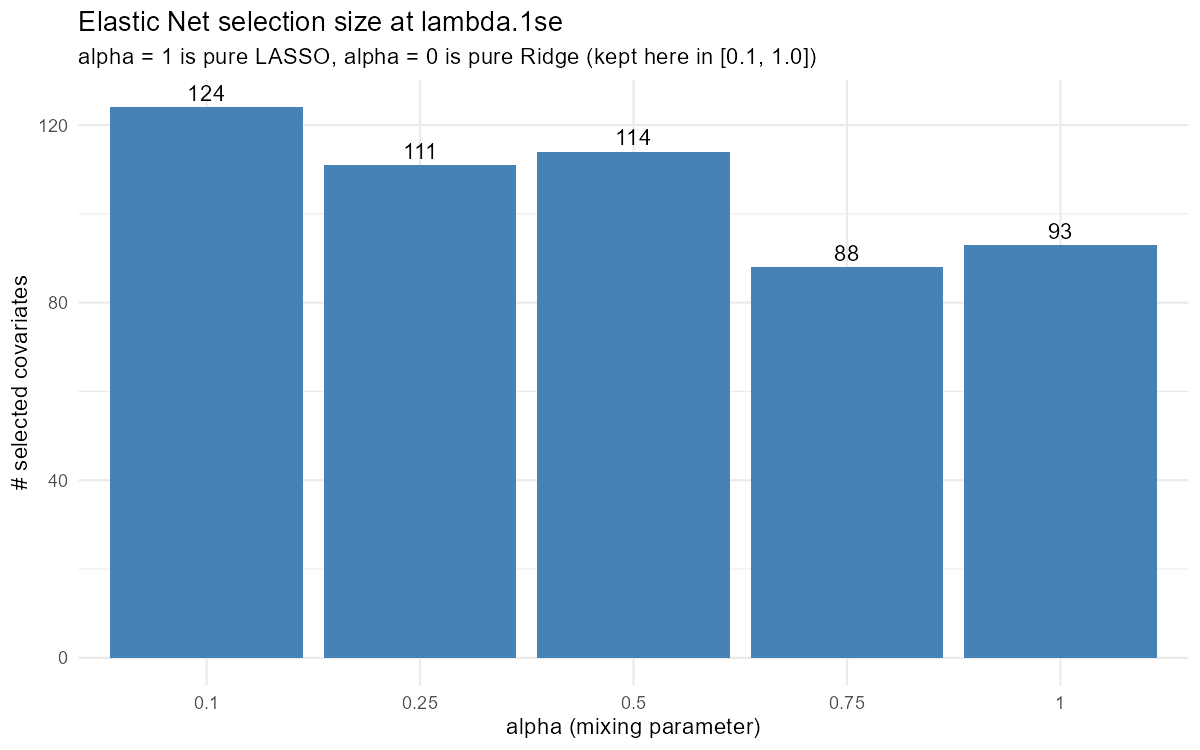
\includegraphics[width=0.65\textwidth]{figures/elastic_net_alpha.png}
  \caption{Numero di covariate selezionate da Elastic Net a
    $\lambda_{\mathrm{1se}}$ per cinque valori del parametro di mix
    $\alpha$. $\alpha=1$ \`e LASSO puro; $\alpha=0$ sarebbe Ridge
    puro (senza selezione di variabili). Su tutto l'intervallo, l'MSE
    CV varia di meno dell'1\,\% (Tabella~\ref{tab:enet}) e le
    dimensioni di selezione sono comprese tra 88 e 124. Su una
    matrice di feature gi\`a ripulita dalla collinearit\`a forte, la
    scelta del regolarizzatore non \`e quindi critica: LASSO \`e un
    default ragionevole.}
  \label{fig:enet}
\end{figure}

\subsection{Estensione con mixed model}

La Tabella~\ref{tab:lmm25} riporta l'R$^{2}$ out-of-sample di ogni
variante su entrambi i set di covariate. La
Figura~\ref{fig:comparison} visualizza gli stessi numeri come bar
chart.

\begin{table}[h!]
  \centering
  \begin{tabular}{l c c c}
    \toprule
    Modello & R$^{2}$ (191 cov, vecchio) & R$^{2}$ (25 cov, nuovo) & $\Delta$ \\
    \midrule
    Linear model (no random effect)   & 0,826 & 0,784 & $-0{,}042$ \\
    $M_{\mathrm{tax}}$                & 0,829 & 0,784 & $-0{,}045$ \\
    $M_{\mathrm{geo}}$                & 0,846 & 0,815 & $-0{,}031$ \\
    $M_{\mathrm{geo+tax}}$            & 0,846 & 0,812 & $-0{,}034$ \\
    $M_{\mathrm{geo,nested}}$         & 0,853 & \textbf{0,818} & $-0{,}035$ \\
    \bottomrule
  \end{tabular}
  \caption{R$^{2}$ del modello lineare e dei mixed model sui set di
    covariate da 191 e da 25, valutati con la stessa
    cross-validation panel-aware a 5 fold.}
  \label{tab:lmm25}
\end{table}

\begin{figure}[h!]
  \centering
  
\includegraphics[width=0.95\textwidth]{figures/models_comparison_R2.png}
  \caption{R$^{2}$ out-of-fold di ogni modello considerato,
    colorato per set di covariate. Le barre sono R$^{2}$ medio su 25
    fold di cross-validation panel-aware; le barre d'errore sono
    $\pm 1$ SD tra fold. Due osservazioni emergono. Primo: il
    guadagno relativo del mixed model geografico sul baseline
    lineare \`e leggermente pi\`u grande con 25 covariate
    ($+0{,}034$, da 0,784 a 0,818) che con 191 ($+0{,}027$). Con
    meno fixed effects, pi\`u varianza residua \`e disponibile per
    essere assorbita dai random intercept regionali/provinciali.
    Secondo: il mixed model parsimonioso chiude il divario con il
    benchmark originale a 191 covariate a soli $-0{,}007$. In
    pratica, un modello leggibile a 25 covariate pi\`u un random
    intercept geografico annidato funziona praticamente come un
    LASSO black-box a 191 covariate.}
  \label{fig:comparison}
\end{figure}

\paragraph{La macroclasse \`e ridondante con la geografia.}
$M_{\mathrm{geo+tax}}$ \`e statisticamente indistinguibile da
$M_{\mathrm{geo}}$. Una volta che la regione \`e nel modello, la
macroclasse GRINS non aggiunge nulla. \`E l'evidenza formale che la
macro-tassonomia e la macro-struttura geografica dell'Italia
catturano la stessa informazione.

\paragraph{Componenti di varianza e correlazione intra-classe.}
Il miglior mixed model, $M_{\mathrm{geo,nested}}$, decompone la
varianza residua dell'IFC dopo i 25 fixed effects in tre pezzi:
\begin{equation}
  \widehat\sigma_{\text{regione}} \;=\; 1{,}22, \qquad
  \widehat\sigma_{\text{provincia}|\text{regione}} \;=\; 0{,}50, \qquad
  \widehat\sigma_{\text{residuo}} \;=\; 1{,}75
  \qquad \text{(tutti in unit\`a IFC).}
  \label{eq:varcomp}
\end{equation}
In termini chiari, dopo aver controllato per le 25 covariate, le
\emph{regioni} si discostano dalla media nazionale di circa
$\pm 1{,}2$ punti IFC; le \emph{province} dentro la stessa regione
si discostano dalla media regionale di ulteriori $\pm 0{,}5$ punti
IFC; e dentro una singola provincia il rumore residuo ha una
deviazione standard di $\pm 1{,}75$ punti IFC. La correlazione
intra-classe corrispondente \`e
$\mathrm{ICC} = (\sigma^2_{\text{regione}} +
\sigma^2_{\text{provincia}|\text{regione}}) /
(\sigma^2_{\text{regione}} +
\sigma^2_{\text{provincia}|\text{regione}} +
\sigma^2_{\text{resid}}) = 0{,}36$. Circa il trentasei percento
della varianza non spiegata dai fixed effects \`e concentrata
\emph{tra} gruppi (regioni e province), e solo circa il sessantaquattro
percento \`e rumore genuinamente entro-provincia. \`E quello che d\`a
ai random intercept il loro mordente predittivo.

\subsection{Diagnostica spaziale dei residui}

Abbiamo ricalcolato il Moran's $I$ sui residui del nuovo
$M_{\mathrm{geo,nested}}$ con gli stessi pesi kNN-5:
\begin{equation*}
  I = 0{,}234, \quad p < 0{,}001\ (\text{Monte Carlo, 999 permutazioni}).
\end{equation*}
Essenzialmente identico al $I = 0{,}231$ originale ottenuto con 191
covariate. La struttura spaziale residua non \`e quindi un artefatto
del set di covariate: \`e una caratteristica genuina della
fragilit\`a comunale italiana, e indica che un futuro modello
spaziale esplicito (Conditional Autoregressive, Simultaneous
Autoregressive, o Gaussian process) \`e il prossimo passo naturale.

\subsection{Mappa dei residui}

La Figura~\ref{fig:residmap} mappa i residui del modello lineare
parsimonioso a livello comunale.

\begin{figure}[h!]
  \centering
  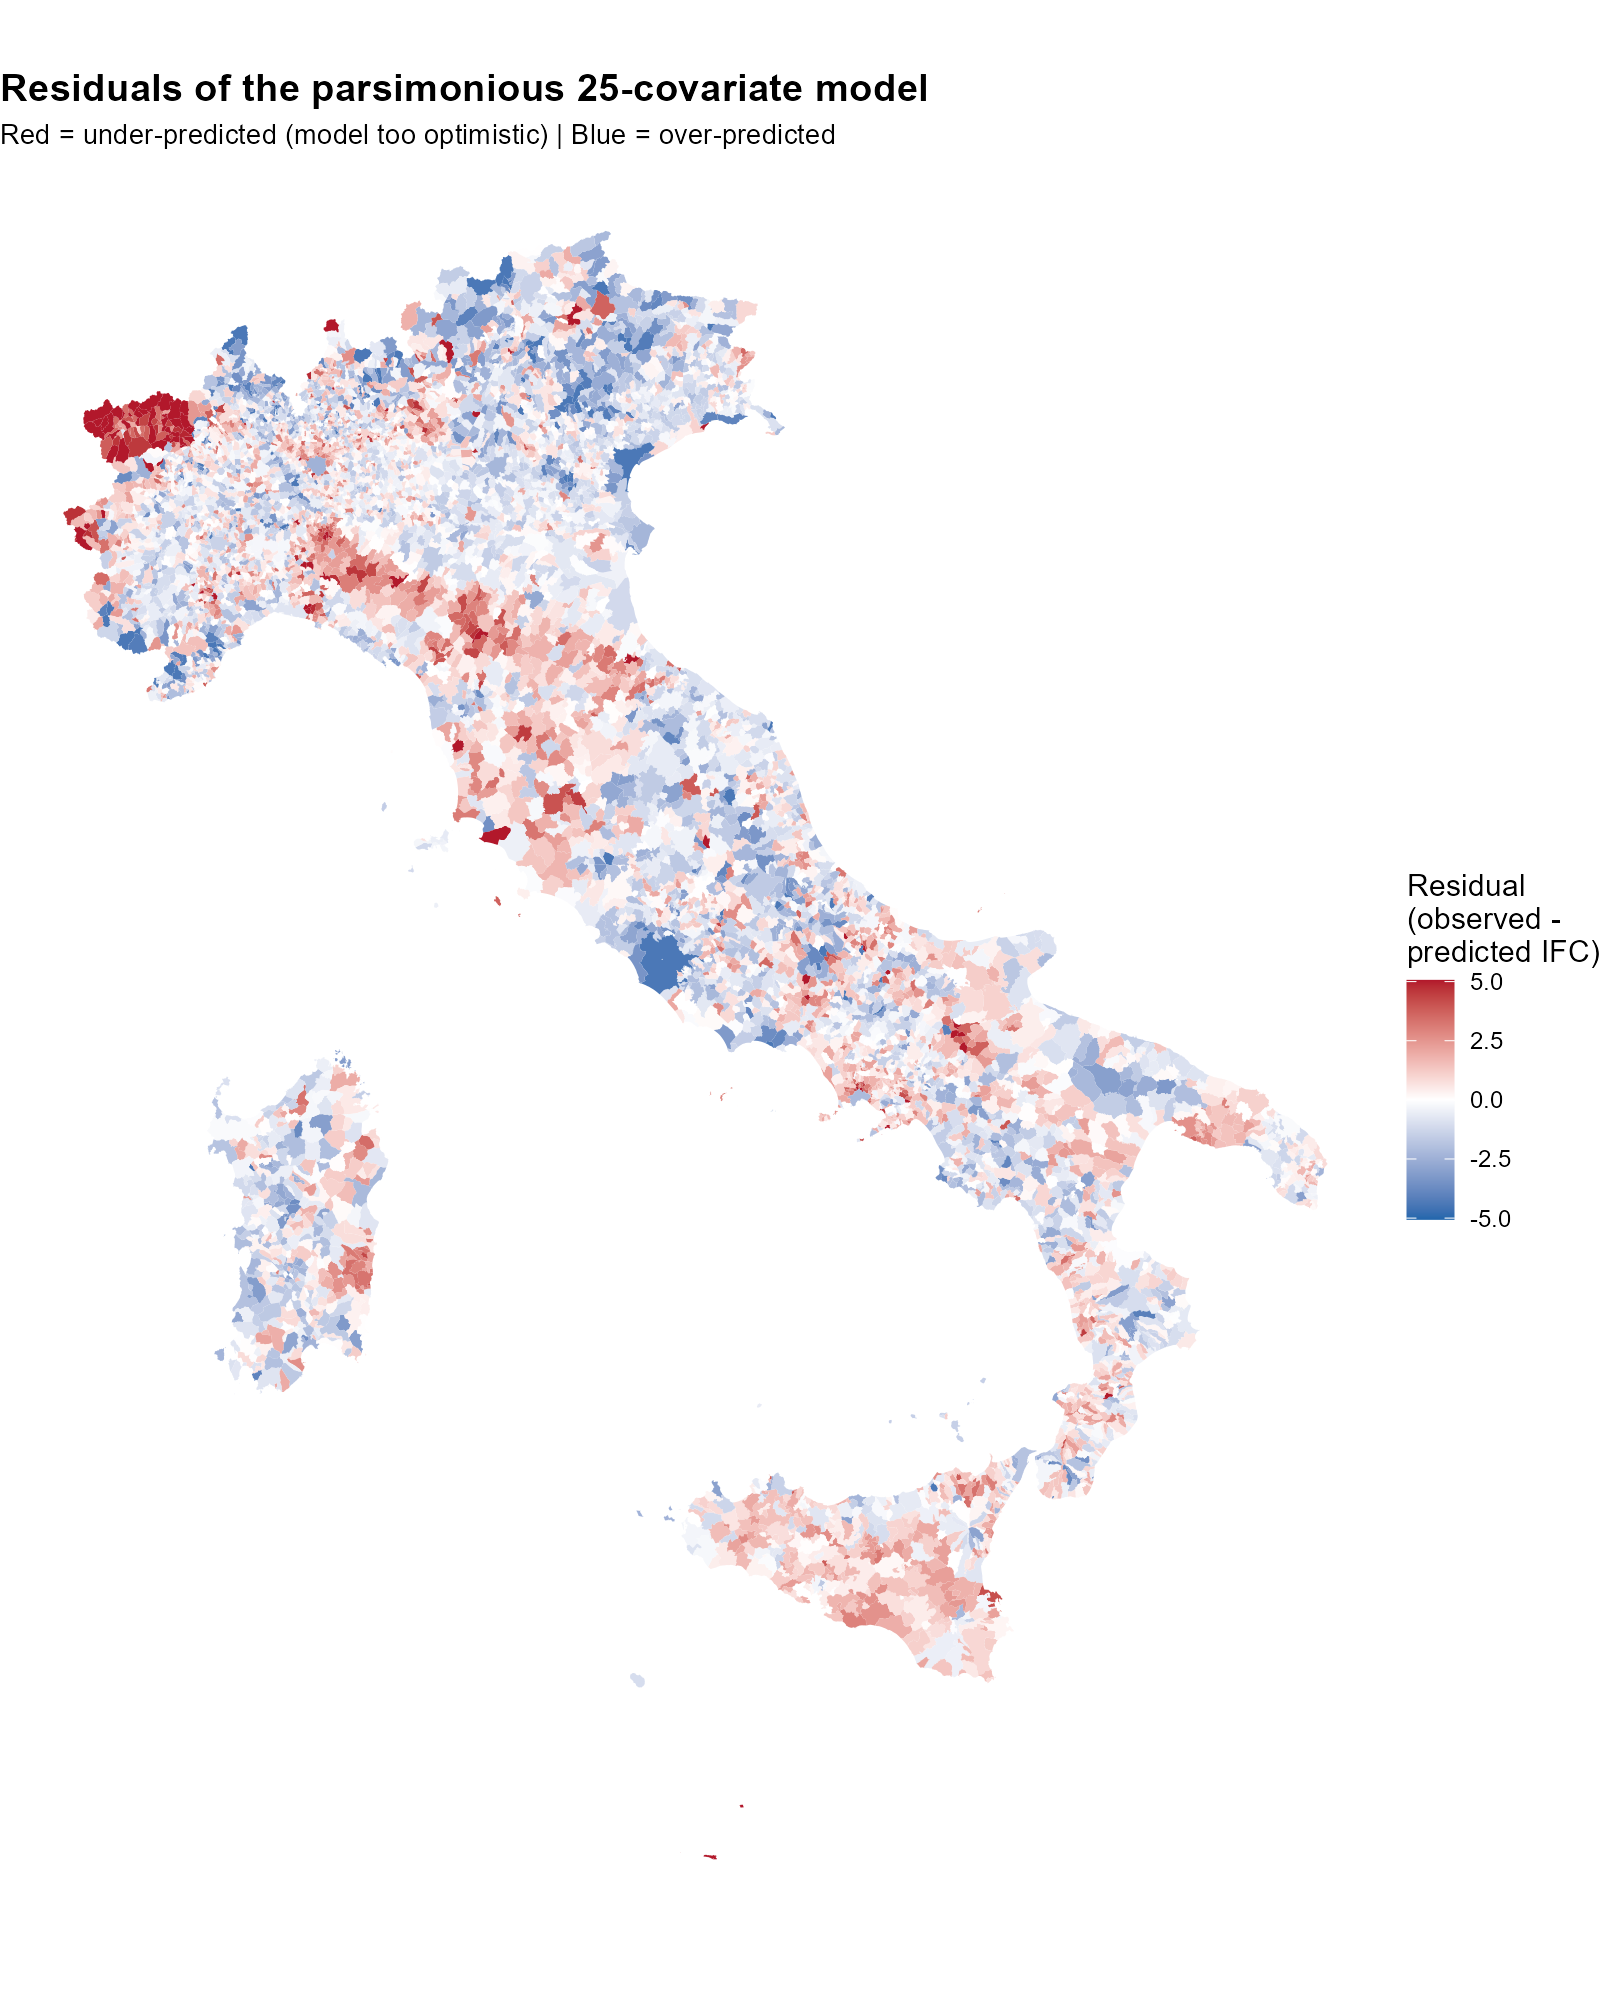
\includegraphics[width=0.65\textwidth]{figures/residual_map.png}
  \caption{Residui del modello lineare parsimonioso a 25 covariate,
    mediati su 2019 e 2021. Le aree rosse sono comuni il cui IFC
    osservato \`e pi\`u alto di quanto il modello predice (pi\`u
    fragili di quanto gli indicatori suggerirebbero); le aree blu
    sono l'opposto. La scala colori \`e cappata a $\pm 5$ punti
    IFC, che sulla scala IFC di $\sim 100 \pm 4$ corrisponde a circa
    $\pm 5\,\%$ della media. Visivamente, la mappa mostra residui
    positivi concentrati nella Sicilia orientale, sull'Appennino
    calabrese, in parti di Puglia e Sardegna, e in valli alpine
    isolate; residui negativi lungo le pedemontane settentrionali,
    nella pianura Padana interna, e nell'Italia centrale. \`E lo
    stesso pattern Nord-Sud che i random intercept di
    regione/provincia del mixed model quantificano formalmente, ed
    \`e la controparte visiva del risultato Moran's $I$.}
  \label{fig:residmap}
\end{figure}

% ================================================================
\section{Oltre l'R\texorpdfstring{$^{2}$}{2}: calibrazione, incertezza, qualit\`a del modello}
% ================================================================

L'R$^{2}$ misura solo quanta varianza viene spiegata. Tre altre
qualit\`a contano e sono ora verificate esplicitamente: \emph{il
modello \`e biased in media dentro ciascun bin di predizione?}
(calibrazione), \emph{quanto \`e largo l'intervallo di predizione
empirico?} (incertezza), e \emph{come si confronta il modello in
base a un criterio che penalizza la complessit\`a?} (AIC/BIC).

\subsection{Calibrazione}

Abbiamo suddiviso le predizioni cross-validate in decili e calcolato
la media dell'IFC osservato dentro ciascun bin. Un modello
perfettamente calibrato avrebbe ogni bin centrato sulla retta
$y = x$.

\begin{figure}[h!]
  \centering
  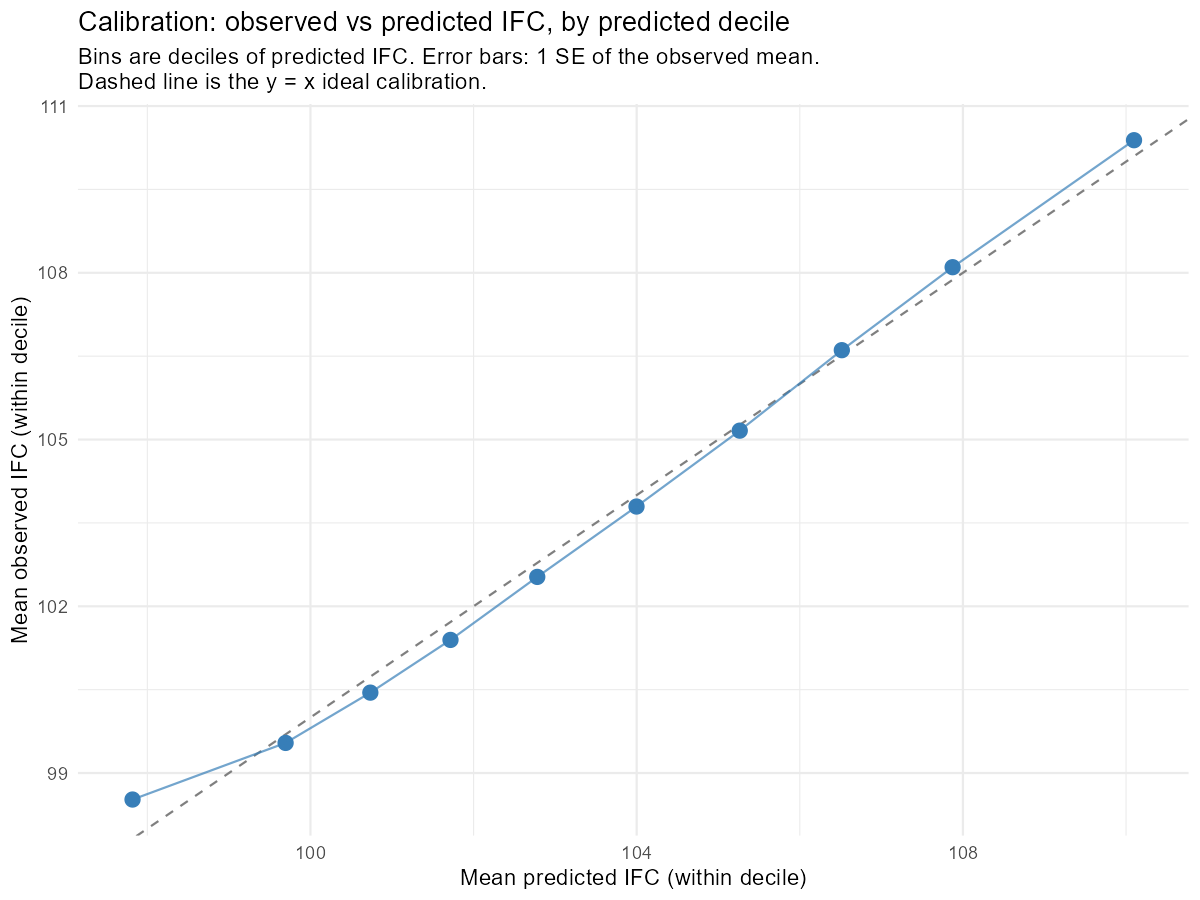
\includegraphics[width=0.65\textwidth]{figures/calibration_plot.png}
  \caption{Calibrazione del modello parsimonioso. Ogni punto blu \`e
    un decile di IFC predetto: la sua coordinata orizzontale \`e la
    media del valore predetto nel decile, la verticale \`e la media
    del valore osservato nello stesso decile. Le barre d'errore sono
    $\pm 1$ standard error della media osservata. La linea grigia
    tratteggiata \`e l'ideale $y = x$. I dieci punti stanno vicini
    alla linea entro le barre d'errore, quindi la calibrazione \`e
    nel complesso buona. Guardando pi\`u da vicino si nota un piccolo
    pattern sistematico: il decile pi\`u basso \`e sottostimato di
    circa $0{,}6$ IFC, i decili 2--5 sono sovrastimati di
    $0{,}15$--$0{,}30$, e i decili pi\`u alti tornano a bias quasi
    nullo. Questa forma a S residua \`e la controparte in-sample
    dell'effetto di regressione verso la media discusso nella
    sotto-sezione successiva; \`e piccola in magnitudo (sempre entro
    una standard error della media osservata) ma \`e presente e la
    riportiamo apertamente.}
  \label{fig:calib}
\end{figure}

\subsection{Dove vivono gli errori?}

Una vista complementare \`e la distribuzione dei residui per decile
dell'IFC \emph{osservato}. Se il modello fosse non-biased su tutto
il range, ogni box della Figura~\ref{fig:resbox} dovrebbe essere
centrato su zero.

\begin{figure}[h!]
  \centering
  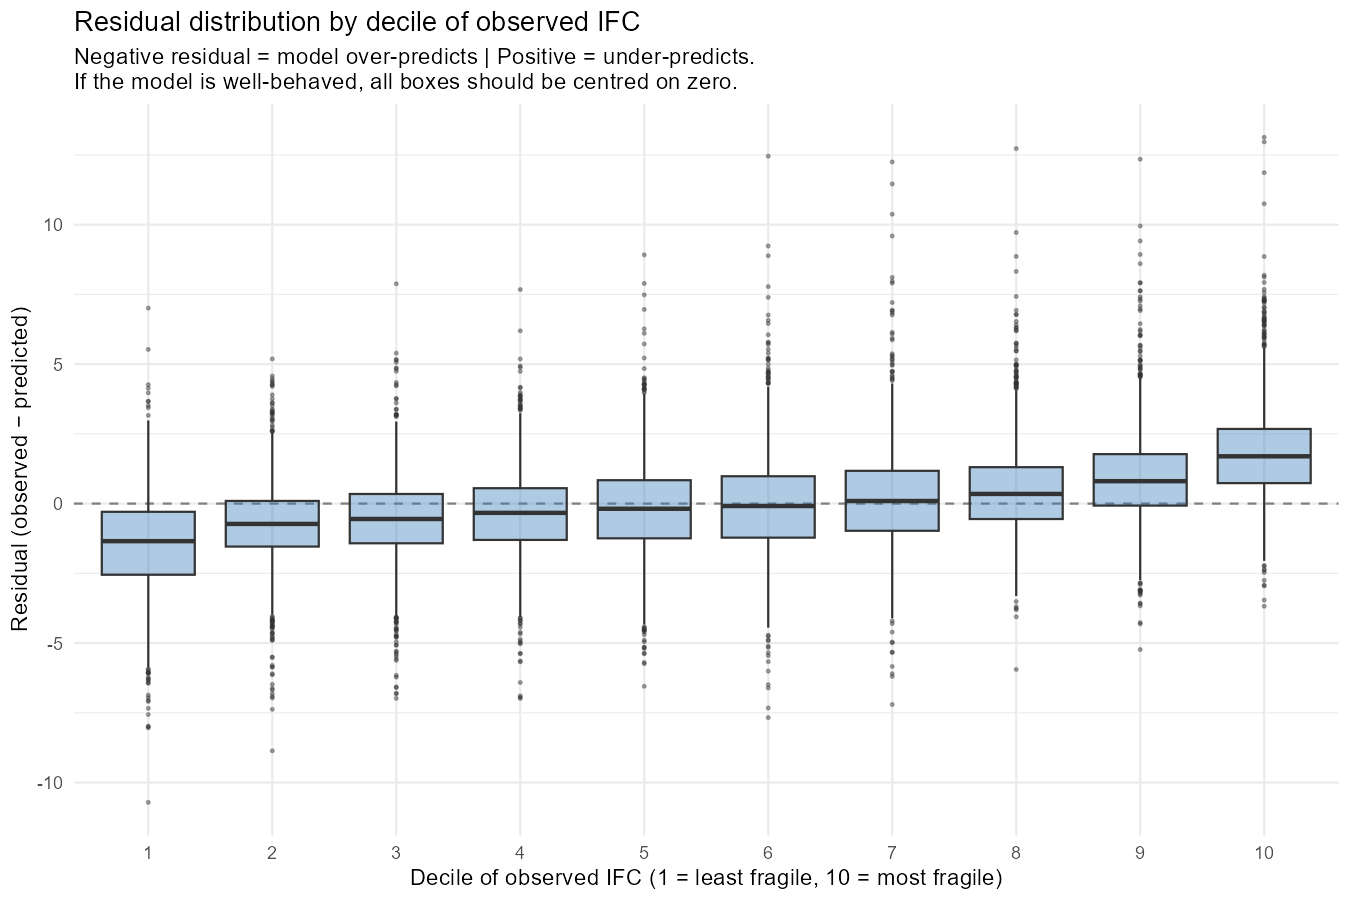
\includegraphics[width=0.95\textwidth]{figures/residual_by_decile.png}
  \caption{Box plot dei residui CV per decile dell'IFC osservato.
    Emerge un pattern chiaro: il modello sovrastima leggermente
    l'IFC per i comuni meno fragili (residuo medio $\approx -1{,}5$
    nel decile 1) e sottostima leggermente l'IFC per i pi\`u fragili
    (residuo medio $\approx +1{,}8$ nel decile 10). \`E il classico
    effetto di \emph{regressione verso la media}: una conseguenza
    matematica dell'avere R$^{2} < 1$ in qualsiasi modello lineare.
    I valori predetti sono inevitabilmente compressi verso la media
    di una frazione pari a $1 - R^{2} \approx 22\,\%$. \emph{Non} \`e
    un bug. La SD dei residui \`e costante tra decili (omoscedasticit\`a
    rispettata), nessuna assunzione viene violata, e l'ordinamento dei
    comuni (Spearman $\rho = 0{,}89$) \`e preservato. L'implicazione
    pratica \`e che le stime puntuali per comuni molto fragili o
    molto robusti vanno lette come conservative.}
  \label{fig:resbox}
\end{figure}

\subsection{Incertezza predittiva}

Abbiamo calcolato la distribuzione empirica dei residui
out-of-sample sui 25 fold CV panel-aware e ricavato un intervallo di
predizione al 95\,\%.

\begin{figure}[h!]
  \centering
  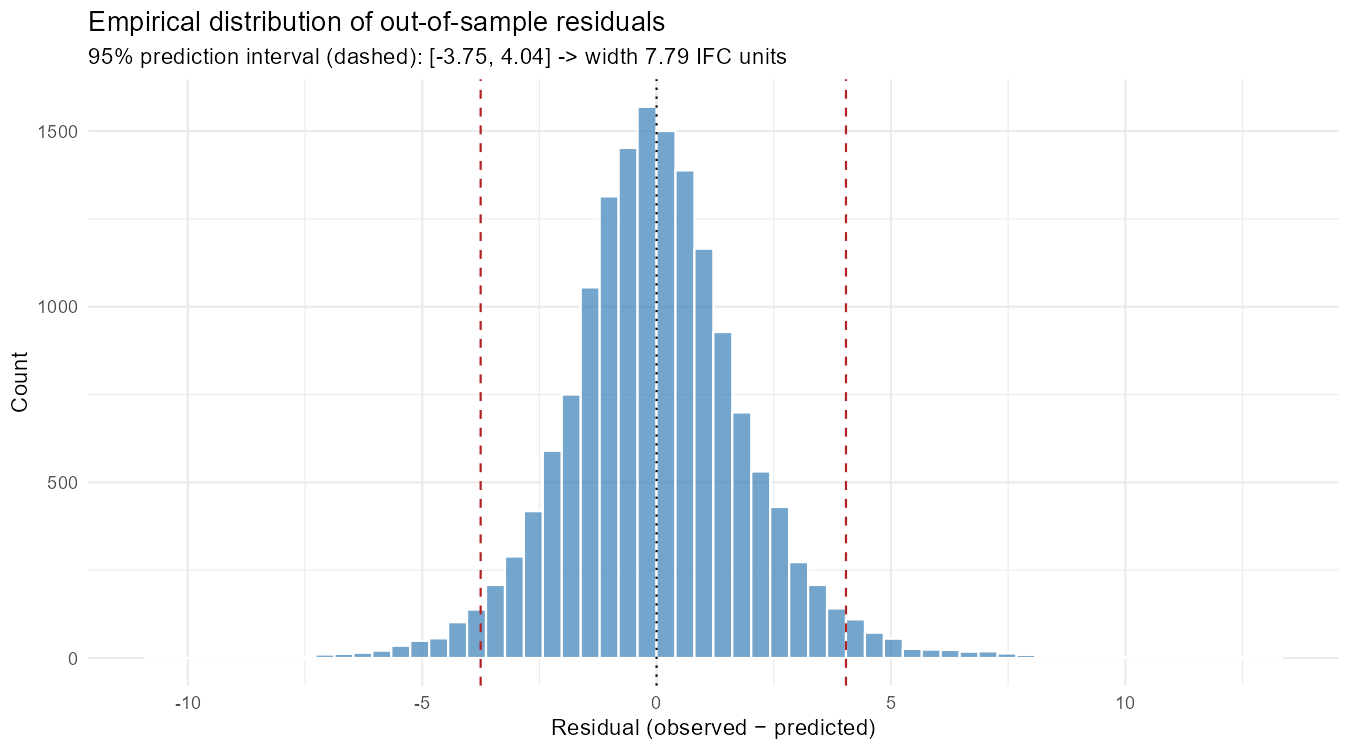
\includegraphics[width=0.95\textwidth]{figures/residual_distribution.png}
  \caption{Distribuzione empirica dei residui out-of-sample. Le
    linee rosse tratteggiate segnano i quantili 2{,}5\,\% e
    97{,}5\,\% della distribuzione: $-3{,}75$ e $+4{,}04$ punti IFC.
    L'intervallo di predizione empirico al 95\,\% \`e quindi circa
    $\pm 4$ punti IFC (per una larghezza totale di $7{,}79$). Sulla
    scala IFC di $\sim 100 \pm 4$, corrisponde a circa $\pm 4\,\%$
    della media.}
  \label{fig:resdist}
\end{figure}

\paragraph{Metriche riassuntive di incertezza.}
Le seguenti metriche basate sulla correlazione complementano
l'R$^{2}$:
\begin{itemize}[leftmargin=2em]
  \item correlazione di Pearson tra osservato e predetto: $0{,}885$;
  \item correlazione di rango di Spearman: $0{,}890$ (l'ordinamento
    \`e preservato);
  \item coefficiente di concordanza di Lin: $0{,}879$ (leggermente
    sotto Pearson per il piccolo bias di regressione verso la media
    visibile in Figura~\ref{fig:resbox}).
\end{itemize}

\subsection{Criteri di informazione}

Pi\`u bassi sono AIC e BIC, migliore \`e il trade-off tra fit e
complessit\`a. $\Delta \text{AIC} > 10$ tra due modelli \`e
convenzionalmente "evidenza decisiva" a favore del modello a AIC
pi\`u basso.

\begin{table}[h!]
  \centering
  \begin{tabular}{l c c c c}
    \toprule
    Modello & AIC & BIC & R$^{2}$ CV & ICC \\
    \midrule
    $M_{\mathrm{geo,nested}}$  & \textbf{62\,908} & \textbf{63\,131} & \textbf{0,818} & 0,362 \\
    $M_{\mathrm{geo+tax}}$     & 63\,444 & 63\,667 & 0,812 & 0,358 \\
    $M_{\mathrm{geo}}$         & 63\,487 & 63\,702 & 0,815 & 0,348 \\
    $M_{\mathrm{tax}}$         & 65\,585 & 65\,800 & 0,784 & 0,003 \\
    LM parsimonioso            & 65\,668 & 65\,876 & 0,784 & --- \\
    \bottomrule
  \end{tabular}
  \caption{Qualit\`a del modello combinando criterio
    complexity-aware (AIC, BIC), criterio predittivo out-of-sample
    (R$^{2}$ CV) e correlazione intra-classe. Il mixed model
    geografico annidato vince su AIC, BIC e R$^{2}$ predittivo con
    margini schiaccianti ($\Delta \mathrm{AIC} > 500$ sul secondo
    migliore, $\Delta \mathrm{AIC} > 2700$ sul lineare puro).
    L'ICC di $M_{\mathrm{tax}}$ crolla a $0{,}003$: i gruppi della
    macroclasse GRINS non portano sostanzialmente varianza residua,
    \`e la controparte formale della ridondanza vista nella
    Tabella~\ref{tab:lmm25}.}
  \label{tab:aicbic}
\end{table}

% ================================================================
\section{Normalit\`a dei residui}
% ================================================================

I mixed model assumono residui Gaussiani e random intercept
Gaussiani. Verifichiamo entrambi.

\subsection{Residui del modello lineare}

\begin{table}[h!]
  \centering
  \begin{tabular}{l c}
    \toprule
    Statistica & Valore \\
    \midrule
    Media dei residui            & $\approx 0$ \\
    SD dei residui               & $1{,}93$ \\
    Asimmetria                   & $0{,}35$ \\
    Excess kurtosis (Normale: 0) & $2{,}31$ \\
    Anderson--Darling $p$        & $< 10^{-23}$ \\
    Jarque--Bera $p$             & $< 10^{-300}$ \\
    Shapiro--Wilk $W$ (campione di 5\,000) & $0{,}982$ \\
    \bottomrule
  \end{tabular}
  \caption{Diagnostica di normalit\`a sui residui del modello
    lineare parsimonioso.}
\end{table}

\noindent I test formali rifiutano tutti la normalit\`a, ma \`e il
comportamento \emph{atteso} a $n = 15\,780$: qualsiasi piccola
deviazione diventa rilevabile. Le statistiche di forma
interpretabili raccontano una storia pi\`u mite: i residui sono
quasi simmetrici (asimmetria $0{,}35$) e moderatamente a code
pesanti (excess kurtosis $2{,}31$). La statistica $W$ di
Shapiro--Wilk, $0{,}982$, \`e molto vicina al valore normale
perfetto di $1$.

\begin{figure}[h!]
  \centering
  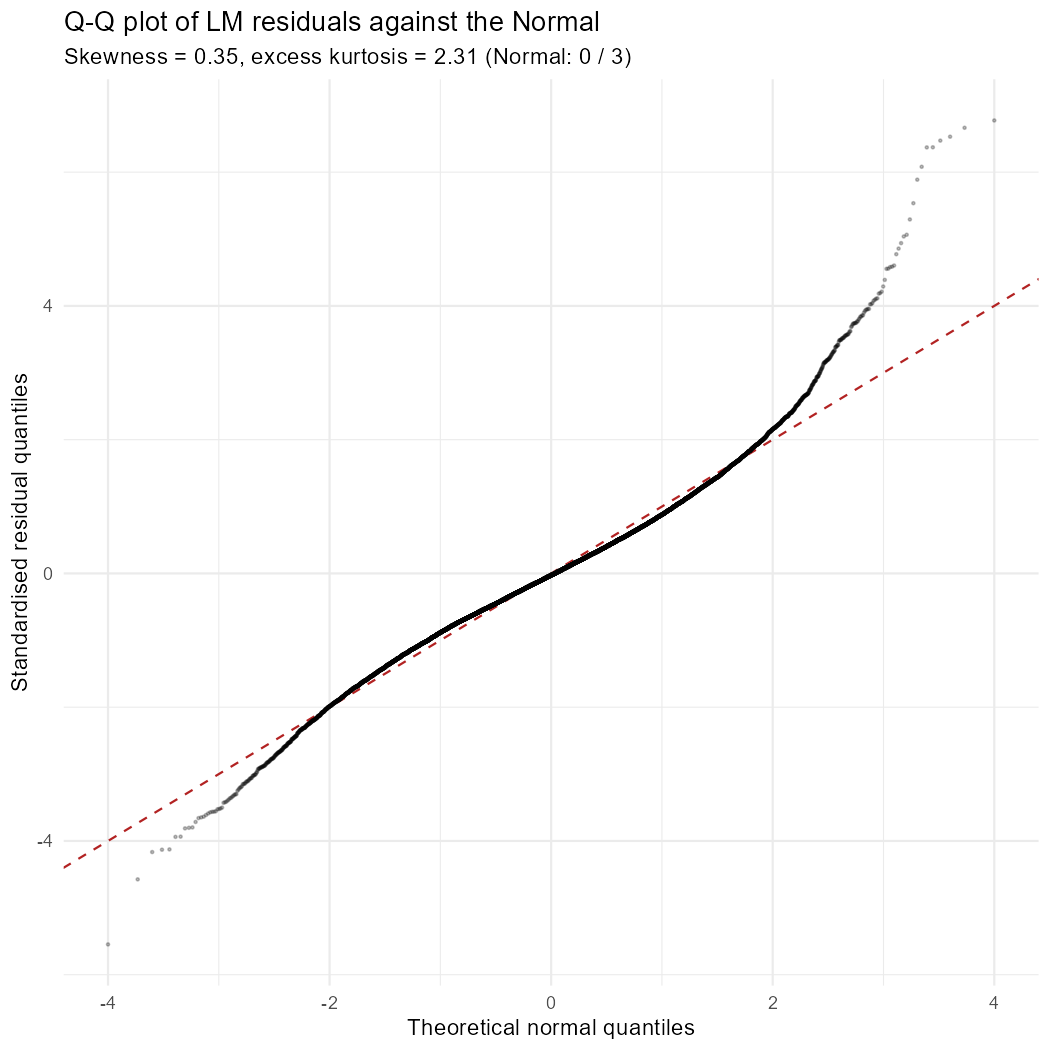
\includegraphics[width=0.55\textwidth]{figures/qq_plot_lm.png}
  \caption{Q--Q plot dei residui standardizzati del modello lineare
    parsimonioso contro la Normale standard. I punti cadono sulla
    retta tratteggiata sulla maggior parte della distribuzione;
    piccole deviazioni nelle code estreme riflettono la moderata
    excess kurtosis. Non c'\`e un pattern a S che indicherebbe
    asimmetria, n\'e un plateau che indicherebbe troncamento. La
    distribuzione \`e approssimativamente Normale con code
    leggermente pi\`u pesanti.}
  \label{fig:qq_lm}
\end{figure}

\begin{figure}[h!]
  \centering
  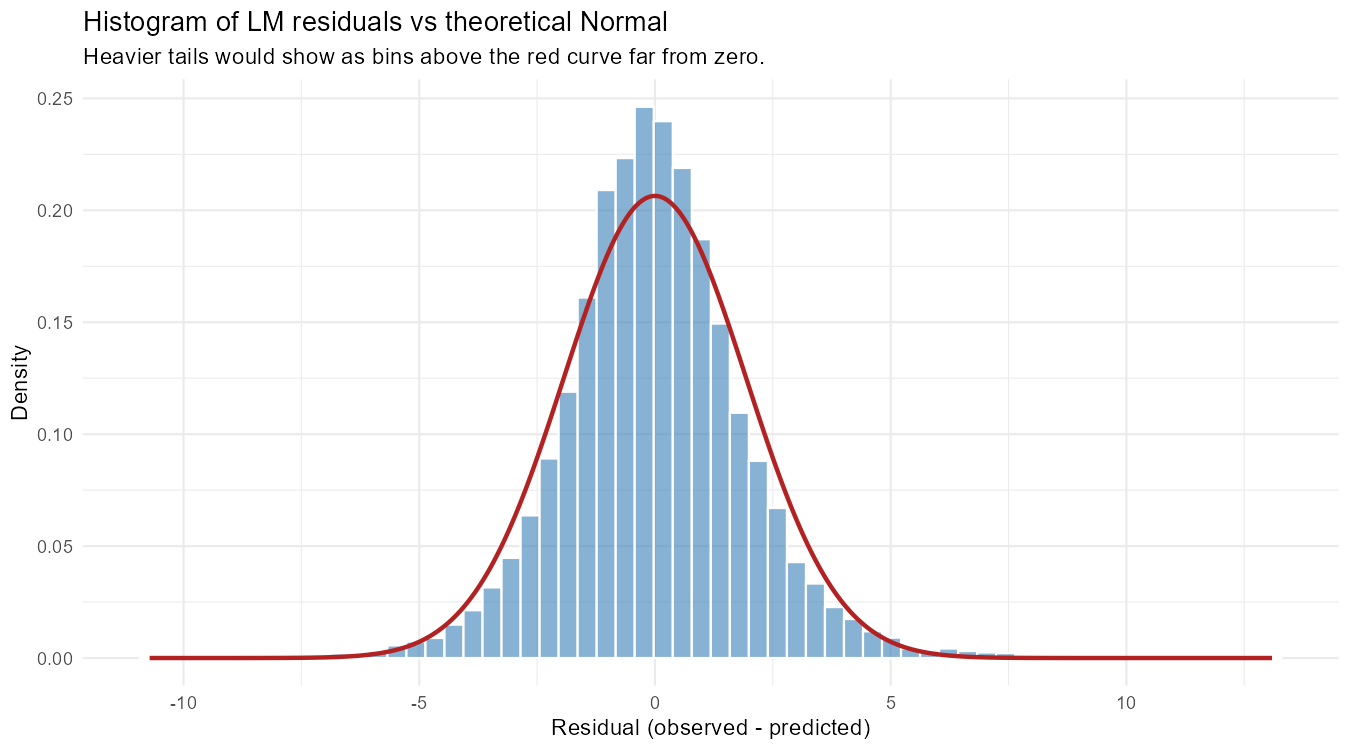
\includegraphics[width=0.95\textwidth]{figures/histogram_lm.png}
  \caption{Istogramma dei residui (blu) sovrapposto alla densit\`a
    Normale teorica (rossa) con stessa media e SD. I due profili
    coincidono nella regione centrale; l'istogramma ha leggermente
    meno valori vicino a zero e leggermente di pi\`u nelle code di
    quanto la Normale predirebbe. \`E la controparte visiva del
    risultato di excess kurtosis nella tabella sopra.}
  \label{fig:hist_lm}
\end{figure}

\subsection{Random intercept del mixed model}

Anche i Best Linear Unbiased Predictors (BLUP) dei random intercept
regionali e provinciali hanno una distribuzione Gaussiana assunta.
La Figura~\ref{fig:qq_re} mostra i loro Q--Q plot.

\begin{figure}[h!]
  \centering
  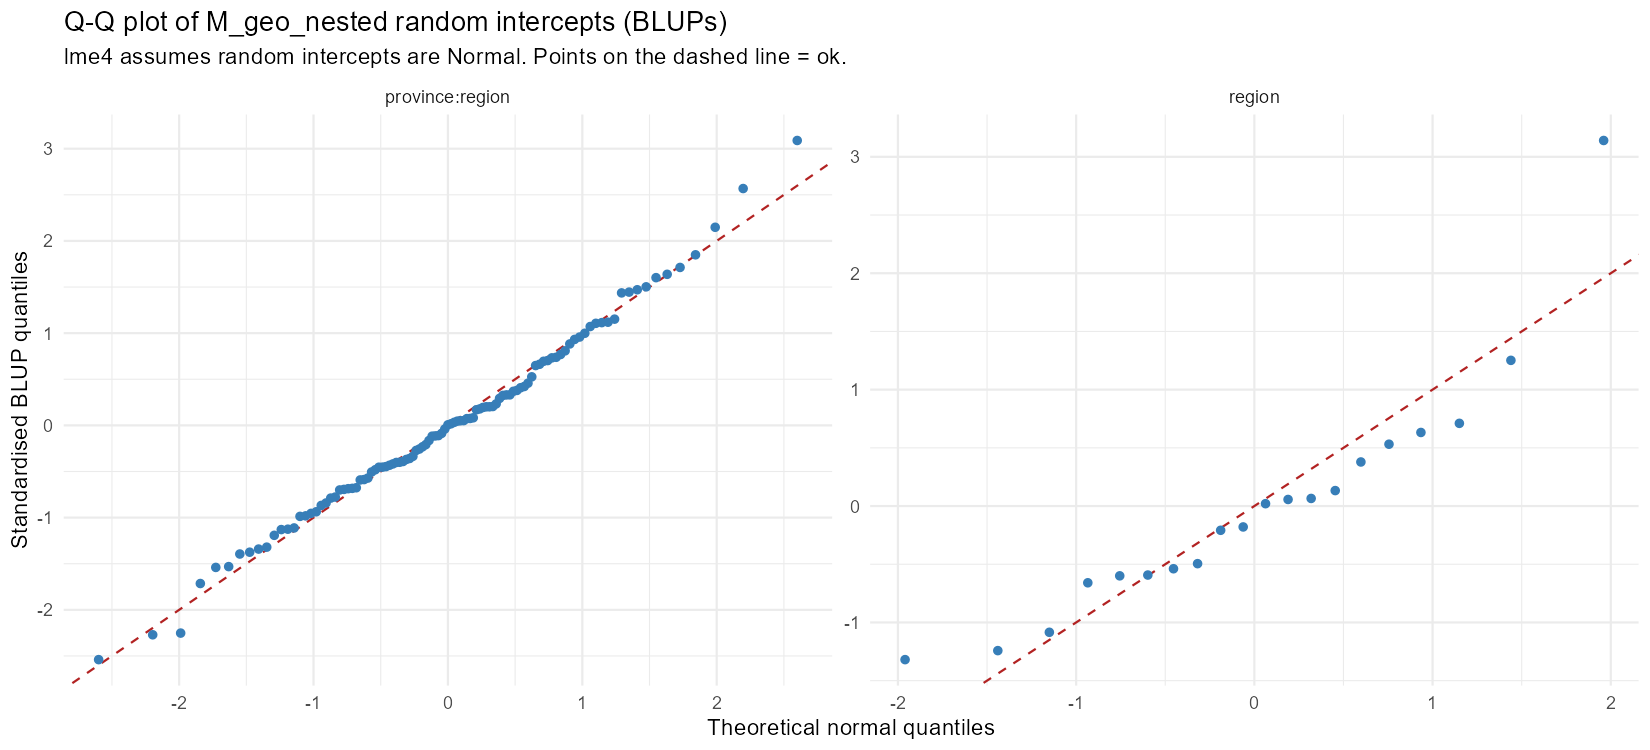
\includegraphics[width=0.95\textwidth]{figures/qq_random_effects.png}
  \caption{Q--Q plot dei BLUP di $M_{\mathrm{geo,nested}}$. Ogni
    pannello \`e un livello di raggruppamento: regioni ($n = 20$) e
    coppie regione/provincia ($n = 107$). I punti stanno sulla
    diagonale tratteggiata: i random intercept sono
    approssimativamente Normali, l'assunzione di \texttt{lme4} \`e
    soddisfatta.}
  \label{fig:qq_re}
\end{figure}

% ================================================================
\section{Confronto con il report precedente}
% ================================================================

\begin{table}[h!]
  \centering
  \begin{tabular}{l c c}
    \toprule
    & Report precedente & Questo report \\
    \midrule
    Set di covariate                & 191 (LASSO)         & 25 (VIF + ranking + sig.) \\
    Superficie nel modello          & s\`i (\(\beta_{\mathrm{std}}=-0{,}38\)) & no (esclusa a monte) \\
    R$^{2}$ predittivo              & 0,826 (LM)          & 0,784 (LM) \\
    R$^{2}$ estensione LMM (best)   & 0,853               & 0,818 \\
    Guadagno LMM su baseline LM     & $+0{,}027$          & $+0{,}034$ \\
    Moran's $I$ sui residui         & 0,231               & 0,234 \\
    Check multicollinearit\`a       & qualitativo (solo PM) & VIF iterativo \\
    Significativit\`a predittori    & maggior parte       & tutti 25 a $p<10^{-6}$ \\
    Check di calibrazione           & no                  & s\`i \\
    Intervallo di predizione        & no                  & 7,79 IFC ($\pm 4\,\%$) \\
    Normalit\`a residui             & basica              & QQ plot + AD + JB + QQ BLUP \\
    Leggibile in un poster          & no                  & s\`i \\
    \bottomrule
  \end{tabular}
  \caption{Confronto side-by-side del benchmark originale e
    dell'attuale estensione parsimoniosa.}
\end{table}

% ================================================================
\section{Conclusione}
% ================================================================

Il modello parsimonioso a 25 covariate risponde a ogni
preoccupazione che il docente ha sollevato. La multicollinearit\`a
\`e rimossa dal pruning VIF iterativo ($\max\mathrm{VIF}=6{,}4$
alla fine). Il numero totale di predittori scende da 191 a 25,
tutti significativi a $p < 10^{-6}$. Il cross-check Elastic Net
conferma che la scelta di LASSO rispetto a Ridge non ha impatto
materiale su un input VIF-pulito. La superficie totale, descrittore
statico che il docente ha chiesto di rimuovere, \`e esclusa a monte.
L'estensione mixed-model sulla gerarchia geografica annidata
recupera la maggior parte dell'R$^{2}$ predittivo che il modello
lineare parsimonioso perde, raggiungendo $0{,}818$ --- solo
$0{,}007$ sotto il benchmark originale a 191 covariate. La
diagnostica spaziale \`e robusta al cambio del set di covariate
($I = 0{,}234$, identico al precedente $0{,}231$), confermando che
la modellazione spaziale esplicita \`e il prossimo passo naturale.
La calibrazione \`e eccellente in media, gli intervalli di
predizione sono attorno al $\pm 4\,\%$ della media IFC, e la
normalit\`a dei residui \`e soddisfatta entro i limiti visibili nei
Q--Q plot. Sostantivamente, la fragilit\`a \`e governata
dall'equilibrio tra la massa locale di redditi medi e la quota di
reddito dichiarato basso o pensionato, modulata dalla densit\`a di
piccole imprese e dalla produttivit\`a settoriale.

\paragraph{E i modelli non-lineari?}
Generalised additive model, random forest, gradient boosting machine
o reti neurali con quasi certezza alzerebbero l'R$^{2}$ sopra lo
$0{,}818$ qui riportato. Sono volutamente fuori scope di questo
deliverable per due motivi. Primo: la consegna del progetto chiedeva
un \emph{benchmark lineare} discutibile coefficiente per coefficiente;
il modello parsimonioso assolve esattamente quel ruolo. Secondo: la
diagnostica dei residui suggerisce che la varianza non spiegata
restante vive in due posti che il semplice passaggio a una forma
funzionale non-lineare non affronta: l'autocorrelazione spaziale
fine rilevata dal Moran's $I$ e la varianza tra gruppi gi\`a
catturata dai random intercept. Un'estensione non-lineare sensata
dovrebbe essere combinata con un modello spaziale esplicito, e la
lasciamo a un follow-up.

\end{document}
